\setchapterimage[6cm]{chapter/anime/Kiki.png}

\chapter{Anime: a mysterious and stunning world of Japanese animation\protect\footnotemark}

\labch{anime}

\footnotetext{\href{https://en.wikipedia.org/wiki/Krita\#Mascot}{Kiki}, an anime-styled \href{https://en.wikipedia.org/wiki/Mascot}{mascot} of Krita, free graphical editor. 
Author: \href{https://www.deviantart.com/tysontan/art/The-Magic-Stylus-570566846}{Tyson Tan, DeviantArt / 2015 / Creative Commons Attribution-Share Alike 3.0 Unported License}.}

\marginnote[0.0cm]{Seiyu are the Japanese voice actors. Usually seiyu give voice to the characters of anime, video games, movies, work on the radio and TV. They act as storytellers on radio shows. Moreover, the seiyu's voices are used in advertisements, voice announcements, book audios and for re-sounding. Men and women, adults and children can work as seiyu.}

This chapter is dedicated to \wdqName{anime}{1107} Wikidata object analysis. Using SPARQL queries executed on Wikidata objects of anime type, several tasks were accomplished. The list of seiyu ordered by number of anime voiced by them is shown, the histogram of seiyu that acted in one or more anime is presented, the graph that connects seiyu and anime voiced by them is constructed, the estimate of age of the seiyu's activity is received.

\begin{marginfigure}[0.0cm]
{
	\setlength{\fboxsep}{0pt}%
	\setlength{\fboxrule}{1pt}%
	\fcolorbox{gray}{gray}{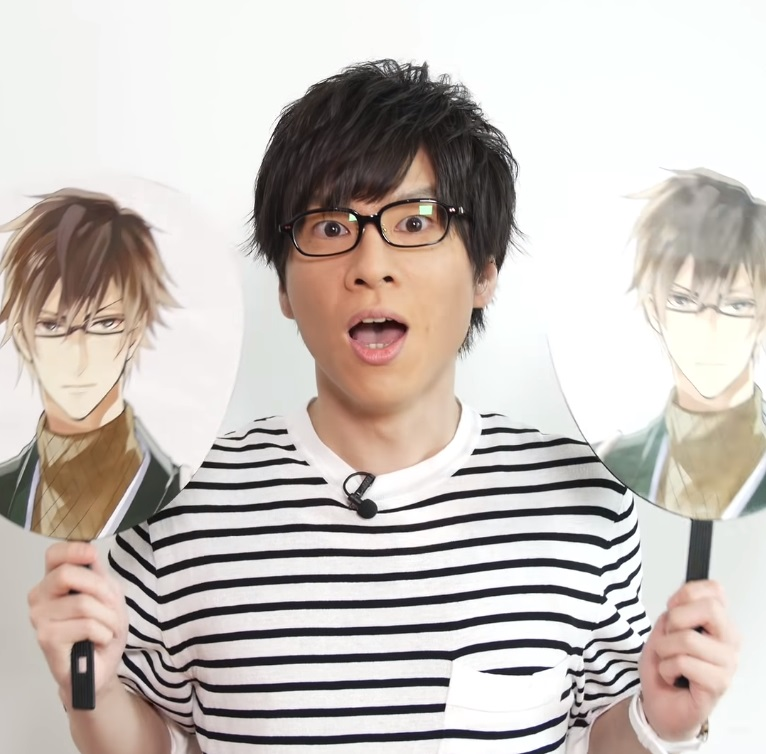
\includegraphics{chapter/anime/seyu.jpg}}
}
\caption
[Seiyu Kenji Akabane, 2021.]
{
Seiyu Kenji Akabane voiced the role of Sasuke Sarutobi in Ikemen Sengoku videogame, 2018.\newline
Wikimedia Commons / numan (CC BY-SA 3.0)
}
\label{fig:seiyu}
\end{marginfigure}

\section{Anime object instances}

Anime is the Japanese animation. It is special because of its visual style, but there are other features that are not that obvious. For instance, anime has a significantly wider variety of genres in comparison to the American and European animation: from family comedies and movies for kids to dramatic stories, whereas in the Western cinema the stories of such genre are mostly shown in the live action movies.

Each anime has its own voice actors. Further, we will call the Japanese voice actors seiyu. In the Japanese animation, the terms \emph{seiyu} and \emph{voice actor} are synonyms. Usually, the word \emph{title} means the certain anime. Generally, \emph{title} means the term which combines different kinds of products, from cinema to novel, that are based on the same literary work which has an exact name.

% analog of wdProperty is needed
In order to work with the anime list from Wikidata, we need to use the \wdqName{anime}{1107} object and the \href{https://www.wikidata.org/wiki/Property:P31}{instance of (P31)} property. Let's get the list of all anime names, without anime subclasses (listing~\protect\ref{lst:anime}).

\begin{lstlisting}[ language=SPARQL, breaklines=true, 
                    caption={List of anime without subclasses.\\\hspace{\textwidth}
                        The result contains \num{683} instances of anime in 2017, 
                        \num{216} instances of anime in 2021.\\\hspace{\textwidth}
                        SPARQL query: \href{https://w.wiki/4ABq}{w.wiki/4ABq}
                        },
                    label=lst:anime,
                    texcl 
                    ]
# List of instances of anime
SELECT ?anime ?animeLabel
WHERE
{
    ?anime wdt:P31 wd:Q1107. # instance of anime
    SERVICE wikibase:label{bd:serviceParam
					     wikibase:language "en,ja"}
}
\end{lstlisting}%

In fact, there are much more anime objects in Wikidata, but they are the instances not of anime, but of its subclasses, such as, for example, \wdqName{anime series}{63952888}. Let's execute the query~\protect\ref{lst:anime_genres} in order to obtain the list of anime genres and the number of anime that correspond to these genres.

\begin{lstlisting}[ language=SPARQL, breaklines=true, 
                    caption={List of genres (subclasses) of anime.\\\hspace{\textwidth}
                        The result contains \num{11} genres of anime in 2021.\\\hspace{\textwidth}
                        SPARQL query: \href{https://w.wiki/4ABt}{w.wiki/4ABt}
                        },
                    label=lst:anime_genres,
                    texcl 
                    ]
# Select anime and its subclasses with number of titles
# corresponding to these subclasses
SELECT ?subAnime ?subAnimeLabel
(COUNT(?subAnimeInstance) AS ?count) WHERE {
  ?subAnime wdt:P279* wd:Q1107.
  ?subAnimeInstance wdt:P31 ?subAnime
  SERVICE wikibase:label { bd:serviceParam wikibase:language "en,ja". }
}
GROUP BY ?subAnime ?subAnimeLabel
ORDER BY DESC(?count)
\end{lstlisting}%

This classification of anime by genres is not perfect because there is a significant skewness to the anime television series: among \num{4875} titles, {2984} are the instances of anime series genre (\num{62,7}\%). Also, some subclasses correspond not to genres, but to the particular anime (i.e., \href{https://w.wiki/3iKe}{Evangelion}).

Let's get the list of all anime names, including the titles that are the instances of anime subclasses, with script~\protect\ref{lst:all_anime_list}.

\begin{lstlisting}[ language=SPARQL, breaklines=true, 
                    caption={List of anime, including the titles that are instances of anime subclasses.\\\hspace{\textwidth}
                        The result contains \num{4875} anime names in 2021.\\\hspace{\textwidth}
                        SPARQL query: \href{https://w.wiki/4ABv}{https://w.wiki/4ABv}
                        },
                    label=lst:all_anime_list,
                    texcl 
                    ]
# List of instances of anime and subclasses of anime
SELECT ?anime ?animeLabel
WHERE
{
    ?anime wdt:P31/wdt:P279* wd:Q1107. # instance of anime with
                                                       # subclasses
    SERVICE wikibase:label { bd:serviceParam wikibase:language "en,ja" }
}
\end{lstlisting}%

Anime that have the most complete information on Wikidata are \wdqName{Gurren Lagann}{4277}, \wdqName{Space Battleship Yamato}{4292}, \wdqName{Project A-ko}{4316}. There are also some anime with many missing properties like \wdqName{Doraemon}{711311}, \wdqName{The Animal Conference on the Environment}{97195557} and \wdqName{Assassins Pride}{96737300}.

% add Prowd link
According to ProWD service, among all the anime titles on Wikidata, \wdqName{Fullmetal Alchemist: The Sacred Star of Milos}{1004318}\footnote{Fullmetal Alchemist: The Sacred Star of Milos is an anime movie which continues the Fullmetal Alchemist anime series. Its main characters are the alchemist brothers who use their magic to fight the criminals and forces of evil.} has the greatest number of properties (\num{24}).